\chapter{Introducción}

Las redes neuronales son un modelo computacional basado en un gran conjunto de neuronas individuales de forma aproximadamente análoga al comportamiento observado en los axones de las neuronas en los cerebros biológicos.

\bigskip

Actualmente existe una gran cantidad de programas que hacen uso de las redes neuronales para toda clase de aplicaciones; desde traducción de texto a clustering de datos.

\bigskip

Una de estas aplicaciones es el reconocimiento óptico de elementos. Concretamente, la base de datos MNIST\footnote{\url{http://yann.lecun.com/exdb/mnist/}} es un conjunto de imágenes con números escritos a mano. Esta base de dato tiene un conjunto de 60,000 imágenes, con un tamaño estándar de 28*28 píxeles cada una, y es la que se utilizará en esta práctica. En la figura \ref{fig:mnist-numbers} puede verse un ejemplo de los números almacenados en esta base de datos.

\bigskip

\begin{figure}[H]
\centering
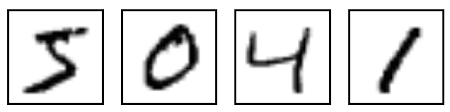
\includegraphics[width=0.6\textwidth]{../images/mnist-numbers}
\caption{Ejemplo de números en la base de datos MNIST}
\label{fig:mnist-numbers}
\end{figure}

\bigskip

Concretamente, se utilizará esta base de datos para entrenar una red neuronal y aplicarla al reconocimiento de estos caracteres, intentado acertar en el mayor número posible.

\bigskip

En esta práctica se podría optar o bien por desarrollar una red neuronal desde 0 o bien por utilizar un framework o conjunto de librerías ya desarrollado. Esta decisión se basará y se justificará en el siguiente capítulo.
\bigskip

\section{Entorno de desarrollo}

Mi ordenador personal, en el cual se ha realizado esta práctica, cuenta con las siguientes características.

\begin{itemize}
  \item \textbf{Sistema operativo}. Ubuntu 18.04.1 LTS (Bionic Beaver)
  \item \textbf{Procesador}. Intel Core i7-6700HQ Quad-Core 2.6GHz
  \item \textbf{Cache}. 6M
  \item \textbf{Memoria RAM}. 8GB DDR4 2,133MHz
  \item \textbf{Tarjeta gráfica}. Sí, pero no recodida por el sistema operativo, por lo que no podrá usarse.
  \item \textbf{Disco duro}. SanDisk SSD Plus 256GB
 \end{itemize}
